\documentclass[conference,11pt]{IEEEtran}
\IEEEoverridecommandlockouts

\usepackage{algorithm}
\usepackage{algpseudocode}
\usepackage{multirow}
\usepackage{multicol}
\usepackage{siunitx}
\usepackage{booktabs}
\usepackage{listings}
\usepackage{stfloats}
\usepackage{midfloat}
\usepackage{color}
\usepackage[table]{xcolor}
\usepackage{lipsum}
\usepackage[utf8x]{inputenc}
\usepackage{float}
\usepackage{bbm}
\usepackage{graphicx}
\usepackage{caption,subcaption}
%\usepackage{amsmath}
\usepackage{amsmath,amsfonts,amssymb}
\usepackage[font={small,it}]{caption}
\usepackage[colorlinks=true,linkcolor=black,anchorcolor=black,citecolor=black,filecolor=black,menucolor=black,runcolor=black,urlcolor=black]{hyperref}
\usepackage{tikz}
\usetikzlibrary{shapes,arrows}
\usepackage{standalone}
\usepackage{balance}
%\usepackage{isomath}
%\renewcommand{\vec}{\mathbfit}
\renewcommand{\vec}[1]{\ensuremath{\boldsymbol{\mathit{#1}}}}

\newtheorem{thm}{Theorem}[section]
\newtheorem{defn}[thm]{Def.}
\newtheorem{propen}[thm]{Prop.}
\newtheorem{cor}[thm]{Cor.}
\renewcommand\IEEEkeywordsname{Keywords}
\def\BibTeX{{\rm B\kern-.05em{\sc i\kern-.025em b}\kern-.08em
		T\kern-.1667em\lower.7ex\hbox{E}\kern-.125emX}}

\title{Short-term Path Planning with Multiple Moving Obstacle Avoidance based on Adaptive MPC}
\author{
	\IEEEauthorblockN{Alberto Franco}
	\IEEEauthorblockA{Department of Information Engineering,\\ Università degli Studi di Padova, Italy\\		 \href{mailto:alberto.franco.3@studenti.unipd.it}{alberto.franco.3@studenti.unipd.it}\\
	\href{mailto:alberto.franco@ua.pt}{alberto.franco@ua.pt}}
	\and
    \IEEEauthorblockN{Vitor Santos}
	\IEEEauthorblockA{Department of Mechanical Engineering,\\ IEETA, Universidade de Aveiro, Portugal\\ \href{mailto:vitor@ua.pt}{vitor@ua.pt}}}
	
\begin{document}
\maketitle
\thispagestyle{plain}
\pagestyle{plain}
\begin{abstract}
	This paper presents a different strategy for a self-driving car short-term path planning among multiple moving obstacles. The main task is to study and implement a motion planning and execution framework in order to make ATLASCAR2 coexist with other moving obstacle vehicles by avoiding collision and overtake them when necessary and possible. The proposed technique, based on the Model Predictive Control paradigm, solves an optimization problem formulated in terms of cost minimization under constraints. Simulation results demonstrate and verify the feasibility and the usefulness of the method considering different scenarios, opening space for real scenario implementation.
\end{abstract}

\section{Introduction}
In robotic research, the problem of navigation is among the most important. Basically, all autonomous mobile robots need some kind of navigation abilities to perform, localization, motion planning and guidance \cite{skoda}.
In the present context, we focus on navigation as a process of planning a path of a mobile robot from its current position to a desired goal location, following the planned path, and avoiding any discovered obstacles along the way \cite{fuzzyMPC} \cite{NONMPC}. The desired paths have to fulfill several conditions to ensure safety and feasibility of the navigation \cite{safety}. Moreover, the paths can be also defined in terms of specifications; for example, short or smooth paths are usually more desirable than long and curved ones in very dynamic environments \cite{archi}. Beyond the path planning, the navigation problem also involves reacting to changes of the environment model. Robots are required to move towards the target in a short time and avoid either static or dynamic obstacles observed by their sensors, which involves efficient path planning and valid obstacle avoidance \cite{MMPC} \cite{autoMPC}. Though these two topics have been well researched, currently, there is no definitive solution to manage the navigation problem within cluttered dynamic environments. In the literature many collision avoidance methods have been developed for wheeled mobile robots; they can be grouped in four categories: graph-search based methods \cite{RRT}, artificial potential field based methods \cite{potential}, meta-heuristic based methods \cite{meta-heuristic} and mathematical optimization based methods \cite{borelli2}.
The latter are very interesting because they offer a systematic and precise way to take vehicle dynamics and safety constraints into account and can produce optimal control inputs. This approach can be used in an closed-loop with a feedback controller for a stronger solution regarding to the Model Predictive Control (MPC). A prior research about obstacle avoidance using MPC in UGVs is dscribed in \cite{borelli} while the applications of nonlinear MPC to ground vehicles is described and evaluated in \cite{nonlinearmpc}.
\begin{figure}[b]
	\centering
	\includegraphics[width=0.6\columnwidth]{./figure/atlascar2.jpg}
	\caption{ATLASCAR2, based on an electric car, a Mitsubishi iMiEV, (adapted from \protect\cite{ricardo}) }
	\label{fig:atlascar2}
\end{figure}
\section{Context and Proposed Solution}
The proposed algorithm was studied for the ATLASCAR project in which the group for Robotics and Automation at the University of Aveiro has setup and adapted a common commercial vehicle to provide a versatile  framework  to  develop  studies  and  research %\cite{atlas}
\cite{atlascar1} \cite{atlascar2}.
Figure \ref{fig:atlascar2} shows the chosen platform for the second generation of ATLASCAR, which is an electric car, a Mitsubishi iMiEV with a range of a \SI{100}{km}.
The fact that the vehicle is electric allows to use the energy stored in the batteries, making it easier to power the sensors installed.

The ATLACAR2 has sensors, such as lidar, that measure the distance to obstacles in front and around the vehicle. The obstacles can be static, such as a large pothole, or moving, such as a moving vehicle on the same or a nearby lane. The most common maneuver from the driver is to temporarily move to another lane, drive past the obstacle, and move back to the original lane afterward. In this case, we want to design an obstacle avoidance system that moves the ATLASCAR2 around a moving obstacle in the lane using throttle and steering angle. This system uses an adaptive Model Predictive Controller that updates both the predictive model and the mixed input/output constraints at each control interval.
%\section{Theoretical background\\ Adaptive Model Predictive Control}
\section{Adaptive Model Predictive Control}
Model Predictive Control is an advanced method that predicts future behavior using a linear-time-invariant (LTI) dynamic model. These predictions are not exact and a good strategy is to make MPC insensitive to prediction errors. If the plant is strongly nonlinear or its characteristics vary dramatically with time, MPC performance might become unacceptable because LTI prediction accuracy degrade \cite{mpctoolbox}. A method that can address this degradation by adapting the prediction model for changing operating conditions is called Adaptive MPC: this control strategy uses a fixed model structure, but allows the model parameters to evolve with time. Ideally, whenever the controller requires a prediction, it uses a model appropriate for the current conditions. At each control interval, the adaptive MPC controller updates the plant model and nominal conditions. Once updated, the model and conditions remain constant over the prediction horizon. The plant model used as the basis for the adaptive MPC must be an LTI discrete-time, state-space model with a structure as follows:
\begin{equation}
\label{eqn:Adaptive_MPC_plant_discrete}
\begin{aligned}
\vec{x}(k+1)&=\vec{A}\vec{x}(k)+ \vec{B}_u \vec{u}(k)+\vec{B}_v \vec{v}(k)+\vec{B}_d \vec{d}(k)\\
\vec{y}(k)&=\vec{C}\vec{x}(k) + \vec{D}_v \vec{v}(k)+ \vec{D}_d \vec{d}(k)
\end{aligned}
\end{equation}
where the matrices \vec{A}, $\vec{B}_u$, $\vec{B}_v$, $\vec{B}_d$, \vec{C}, $\vec{D}_v$ and $\vec{D}_d$ can vary with time. The other parameters in (\ref{eqn:Adaptive_MPC_plant_discrete}) are:
\begin{itemize}
	\item $k$ is the time index/current control interval;
	\item \vec{x} are the plant model states;
	\item \vec{u} are the manipulated inputs that can be adjusted by the MPC controller;
	\item \vec{v} are the measured disturbance inputs;
	\item \vec{d} are the unmeasured disturbance inputs;
	\item \vec{y} are the plant outputs, including both measured (necessary at least one) and unmeasured.
\end{itemize}
In the adaptive MPC control, there are additional requirements for the plant model, like the sample time $T_s$ that has to be constant and identical to the MPC control interval. This control strategy prohibits direct feed-through from any manipulated variable to any plant output. Thus, $\vec{D_v} = \vec{0}$ in the above model.
A traditional MPC controller includes a nominal operating point at which the plant model applies, such as the condition at which you linearize a nonlinear model to obtain the LTI approximation (equilibrium, reference trajectory and the	
most updated value) \cite{mpctoolbox}. In adaptive MPC, as time evolves it should update the nominal operating point to be consistent with the updated plant model. It is possible to rewrite the plant model in terms of deviations from the nominal conditions as follows:
\begin{equation}
\label{eqn:Adaptive_MPC_nominal_condition}
\begin{aligned}
\vec{x}(k+1)&=\overline{\vec{x}}+\vec{A}(\vec{x}(k)-\overline{\vec{x}})+ \vec{B}(\vec{u}_t(k)-\overline{\vec{u}}_t)+\overline{\Delta \vec{x}} \\
\vec{y}(k)&=\overline{\vec{y}}+\vec{C}(\vec{x}(k)-\overline{\vec{x}}) + \vec{D}(\vec{u}_t(k)-\overline{\vec{u}}_t)
\end{aligned}
\end{equation}
where the matrices \vec{A}, \vec{B}, \vec{C} and \vec{D} are updated with respect to time. The other parameters in (\ref{eqn:Adaptive_MPC_nominal_condition}) are:
\begin{itemize}
	\item $\vec{u}_t$ is the combined plant input variable, comprising $\vec{u}$, $\vec{v}$ and $\vec{d}$ variables defined earlier;
	\item $\overline{\vec{x}}$ are the nominal states;
	\item $\overline{\Delta \vec{x}}$ are the nominal state increments;
	\item $\overline{\vec{u}_t}$ and $\overline{\vec{y}}$ are the nominal inputs and outputs.
\end{itemize} 
The adaptive MPC uses a Kalman filter to update its controller states which include the plant, the disturbance and measurement noise model states.
\section{Moving Obstacle Avoidance}
\subsection{Problem Formulation}
The collision avoidance problem is very dependent on the vehicle modeling since it is a requirement for  adaptive MPC law design. Figure \ref{fig:obstacleAvoidance} illustrates a typical scenario of overtaking of a moving obstacle.
%\vspace{-1em}
\begin{figure}[H]
	\centering
	\includegraphics[width=1\columnwidth]{./figure/obstacleAvoidance/obstacleAvoidance.pdf}
%	\vspace{-10pt}
	\caption{Problem description of collision avoidance on a road with only two lanes.}
	\label{fig:obstacleAvoidance}
\end{figure}
%\vspace{-0.5em}
The model used in this paper should take into account the kinematic and dynamic aspects of the vehicle. Here, we present a non linear mathematical model of a vehicle used for the development of a collision avoidance system.
The model has four states and two inputs:
\[ 
\vec{x}=\begin{bmatrix}
   x&y&\theta&v 
  \end{bmatrix}^\intercal
,\qquad 
\vec{u}=\begin{bmatrix}
T&\delta 
\end{bmatrix}^\intercal
\]
where $(x,y)$ are the global coordinates of the contact point between the rear wheel and the ground, $\theta$ is the heading angle of the car body with respect to the $x$-axis and $v$ is the linear speed of the car (positive). The manipulated variables are $T$ the throttle (positive when accelerating/negative when braking) and $\delta$ the steering angle ($0$ when aligned with car, counterclockwise positive). Figure \ref{fig:car_model} illustrates the applied nonlinear bicycle model and the related parameters.
\begin{figure}[H]
	\centering
	\includegraphics[width=0.70\columnwidth]{./figure/car_model.pdf}
%	\vspace{-5pt}
	\caption{Bicycle model of a car, (adapted from \cite{siciliano}).}
	\label{fig:car_model}
\end{figure}
%\vspace{-0.5em}
The ATLASCAR2 can be modeled using the non-linear kinematic bicycle model described by the following equations of motion \cite{safety} \cite{swarms}:
\begin{equation*}
\label{eqn:dynamics_model_obstacle_avoidance}
\left \{ \begin{array}{llll}
\dot{x} = v\cos(\theta)\\
\dot{y} = v\sin(\theta)\\
\dot{\theta} =\dfrac{v}{C_L}\tan(\delta)\\
\dot{v} =0.5 \cdot T
\end{array} 
\right .
\Longrightarrow 
\begin{array}{llll}
\dot{\vec{x}} = \vec{f}(\vec{x},\vec{u})\\
\vec{y} = \vec{g}(\vec{x},\vec{u})
\end{array}
\end{equation*}
where $C_L$ is the car length. In order to simplify the model, it is assumed that only the front wheel can be steered. Moreover, in this paper it is assumed that the ATLASCAR2 does not slip, so any slippage is thus considered as an external disturbance. Under this assumption, the slip angle is zero, meaning that the velocity is directed along the heading of the vehicle. In order to use MPC, the state space model needs to be linearized with a first order approximation and also re-written in a more compact form:
\begin{equation}
\label{eqn:dynamics_model_non_linear}
\begin{array}{llll}
\dot{\vec{x}} = \vec{f}(\vec{x},\vec{u})\\
\vec{y} = \vec{g}(\vec{x},\vec{u})
\end{array} \Longrightarrow
\begin{array}{ll}
\dot{\vec{x}} =\vec{A}_c \vec{x}+ \vec{B}_c \vec{u}\\
\vec{y} =\vec{C}_c \vec{x} + \vec{D}_c \vec{u}
\end{array}
\end{equation}
where the matrices $\vec{A}_c$, $\vec{B}_c$, $\vec{C}_c$ and $\vec{D}_c$ are obtained as follows:
\[ 
\vec{A}_c=\frac{\partial \vec{f}(\vec{x},\vec{u})}{\partial \vec{x}}=\begin{bmatrix}
0&0&-v\sin(\theta)&\cos(\theta)\\
0&0&v\cos(\theta)&\sin(\theta)\\
0&0&0&\tan(\delta)/C_L\\
0&0&0&0
\end{bmatrix},
\]
\[
\vec{B}_c=\frac{\partial \vec{f}(\vec{x},\vec{u})}{\partial \vec{u}}=\begin{bmatrix}
0&0\\
0&0\\
0&\dfrac{v}{C_L}\big(\tan(\delta)^2+1\big)\\
0.5&0
\end{bmatrix},
\]
\[
\vec{C}_c=\frac{\partial \vec{g}(\vec{x},\vec{u})}{\partial \vec{u}} = \mathbf{I}_4, 
\qquad
\vec{D}_c=\frac{\partial \vec{g}(\vec{x},\vec{u})}{\partial \vec{u}}=\mathbf{0}_{4\times2}. 
\]
The simple linearized approximation of the system to describe the dynamics of the ATLASCAR2 will be evaluated at the operating conditions. The system to be controlled is usually modeled by a discrete state-space model in the MPC literature. Therefore, (\ref{eqn:dynamics_model_non_linear})
is transformed into a discrete state-space model to be used by the Model Predictive Controller:
\begin{equation*}
\label{eqn:dynamics_ss_obstacle_avoidance_dis}
	\begin{array}{ll}
	\dot{\vec{x}} =\vec{A}_c \vec{x}+ \vec{B}_c \vec{u}\\
	\vec{y} =\vec{C}_c \vec{x} + \vec{D}_c \vec{u}
	\end{array}
	\Rightarrow
	\begin{array}{rr}
	{\vec{x}}(k+1) =\vec{A}_d \vec{x}(k)+ \vec{B}_d \vec{u}(k)\\
	\vec{y}(k) =\vec{C}_d \vec{x}(k) + \vec{D}_d \vec{u}(k)
	\end{array}
\end{equation*}
where $\vec{A}_d$ and $\vec{B}_d$ are the state and control matrices for the discrete state-space equation, respectively, which can be calculated with the Euler method as
\[
\vec{A}_d = e^{\vec{A}_cT_s},\qquad \vec{B}_d = \int_{kT_s}^{(k+1)T_s} e^{\vec{A}_c[(k+1)T_s-\eta]}\vec{B}_c d\eta
\]
where $T_s$ is the sampling interval for the discrete state-space model. The matrices $\vec{C}_d$ and $\vec{D}_d$ are equivalent to those in the continuous case. For simplicity, we assume that all the states are measurable and the ATLASCAR2 drives east with a constant speed at the nominal operating point. In the scenario that we are going to consider, the road is straight and our vehicle stays in the middle of the center lane when not passing. Without losing generality, the ATLASCAR2 passes an obstacle both to the right and to the left lane depending on where it is placed on the road. We create also a safe zone around the obstacles so that the vehicle does not get too close to the obstacle when passing it.
\subsection{Design of Adaptive Model Predictive Control}
We designed a Model Predictive Controller that can make the ATLASCAR2 maintain a desired velocity and stay in the middle of center lane. We used an Adaptive MPC controller because it handles the nonlinear vehicle dynamics more effectively than a traditional MPC controller; in fact, the latter uses a constant plant model but the former allows us to provide a new plant model at each control interval. Because the new model describes the plant dynamics more accurately at the new operating condition, an adaptive MPC controller performs better than a traditional MPC controller. In practice, at each control interval, the adaptive MPC controller updates the plant model and the nominal conditions. Once updated, the model and the conditions remain constant over the prediction horizon. In motion planning that uses adaptive MPC, it is common to formulate the constrained control problem as a real-time optimization problem subject to hard constraints on plant variables and soft constraints on outputs; at the beginning, we specified the constraints for the manipulated variables: to prevent the ATLASCAR2 from accelerating or decelerating too quickly, we added an hard constraint on the throttle rate of change and another one on the steering angle rate of change. We used an approach that takes advantage of the ability of MPC to handle constraint explicitly. Figure \ref{fig:flowchart} shows a conditional state machine designed for higher-level behavior planning.
\begin{figure}[H]
%\vspace{-1em}
	\centering
%	\includegraphics[width=1\columnwidth]{./figure/flowchart/flowchart.pdf}
	\documentclass[preview,float]{standalone}

\usepackage[latin1]{inputenc}
\usepackage{tikz}
\usetikzlibrary{shapes,arrows}
\begin{document}
	\pagestyle{empty}	
	% Define block styles
	\tikzstyle{decision} = [diamond, draw, fill=blue!10, 
	text width=4.5em, text centered, node distance=3cm, inner sep=0pt]
	\tikzstyle{block} = [rectangle, draw, fill=green!10, 
	text width=5em, text centered, rounded corners, minimum height=4em]
	\tikzstyle{line} = [draw, -latex']
	\tikzstyle{cloud} = [draw, ellipse,fill=red!10, node distance=3cm,
	minimum height=2em]
	
	\begin{tikzpicture}[font={\small\sffamily}, node distance = 3cm, auto, scale=0.75,every node/.style={transform shape}]
	% Place nodes
	\node [decision] (detection) {Rilevato Ostacolo?}; 
	\node [cloud,left of=detection] (start) {Inizio};
	\node [decision,below of=detection] (multiObstacles) {Rilevati Multipli Ostacoli?};
	\node [block,right of=detection] (reference) {Seguire il percorso: attenersi alla corsia};
	\node [block,left of=multiObstacles] (distance) {Calcola la distanza da quello pi� vicino};
	\node [block,right of=multiObstacles] (distances) {Calcola la distanza tra gli ostacoli};
	\node [decision,below of=distances](space) {Spazio libero per sorpassare?};
	\node [block,right of=space,node distance=3.3cm](braking){Frenata/ Velocit� Ostacolo};
	\node [block,below of=space](free){Sorpasso nella corsia libera};
	\node [decision,below of=distance,node distance=2.5cm] (decisionOvertaking) {A sinistra rispetto al veicolo?};
	\node [block, below of=decisionOvertaking,node distance=2.5cm] (rightOver) {Sorpasso a Destra};     
	\node [block, right of=decisionOvertaking] (leftOver) {Sorpasso a Sinistra}; 
	
	%  \node [block] (init) {initialize model};
	% \node [cloud, left of=init] (expert) {expert};
	% \node [cloud, right of=init] (system) {system};
	% \node [block, below of=init] (identify) {identify candidate models};
	%    \node [block, below of=identify] (evaluate) {evaluate candidate models};
	%   \node [block, left of=evaluate, node distance=3cm] (update) {update model};
	%  \node [decision, below of=evaluate] (decide) {is best candidate better?};
	% \node [block, below of=decide, node distance=3cm] (stop) {stop};
	% Draw edges
	\path [line] (start) -- (detection);
	\path [line] (detection) -- node {si} (multiObstacles);
	\path [line] (detection) -- node {no} (reference);
	\path [line] (multiObstacles) -- node {no} (distance);
	\path [line] (multiObstacles) -- node {si} (distances);
	\path [line] (distances)--(space);
	\path [line] (space) -- node{no}(braking);
	\path [line] (space) -- node{si} (free);
	\path [line] (braking) |- (distances);
	\path [line] (distance) -- (decisionOvertaking);
	\path [line] (decisionOvertaking) -- node {no}(leftOver);
	\path [line] (decisionOvertaking) -- node{si} (rightOver);
	\end{tikzpicture}
\end{document}
%	\vspace{-15pt}
	\caption{Behaviour planning conditional flowchart.}
	\label{fig:flowchart}
\end{figure}
%\vspace{-15pt}
When an obstacle is detected, it defines an area on the road (in terms of constraints) that the ATLASCAR2 must not enter during the prediction horizon. At the next control interval the area is redefined based on the new positions of the vehicle and the obstacle until passing is completed.
To define the area to avoid, we used the following mixed Input/Output constraints:
\begin{equation*}
	\label{eqn:mixed_IO_constraints}
	\vec{E}\vec{u}+\vec{F}\vec{y}\leq \vec{G}
\end{equation*}
where $\vec{u}$ and $\vec{y}$ are respectively the manipulated variable vector and the output variable vector, while $\vec{E},\vec{F},\vec{G}$ are the constraint matrices that can be updated when the controller is running. Five constraints were defined:
\begin{enumerate}
	\item upper bound on the $y$-coordinate (left boundary of the road);
	\item lower bound on the $y$-coordinate (right boundary of the road);
	\item constraint for obstacle avoidance; although no obstacle is considered in the nominal condition, we must add this virtual constraint here because we cannot change the dimensions of the constraint matrices at run time;
	\item upper bound on the $x$-coordinate (position of the closest obstacle);
	\item lower bound on the $x$-coordinate (position of the ATLASCAR2).
\end{enumerate}
The matrices for the above inequality are the following:
\[
\vec{E}= 
\begin{bmatrix}
0&0\\
0&0\\
0&0\\
0&0\\
0&0
\end{bmatrix},
\;
\vec{F}=\begin{bmatrix}
0&1&0&0\\
0&-1&0&0\\
cS&-1&0&0\\
1&0&0&0\\
-1&0&0&0\\
\end{bmatrix},\;
\vec{G}=
\begin{bmatrix}
W/2\\W/2\\-cI\\x_{\max}\\x_{\min}
\end{bmatrix}
\]
where $W$ is the width of the road, $cI$ and $cS$ are the required parameters such that the ATLASCAR2 must be above the line formed from the vehicle to safe zone corner for left/right passing and finally $x_{\max}$ represents the position of the closest obstacle in the case there is not free space for the overtaking (otherwise $x_{\max}=+\infty$) while $x_{\min}$ depicts the location of our vehicle. Figure \ref{fig:constraint} illustrates the constraints that are computed at each $T_s$ in the case of a left overtaking.
\begin{figure}[H]
%\vspace{-12pt}
	\centering
	\includegraphics[width=0.9\columnwidth]{./figure/constraint/constraint.pdf}
%	\input{./figure/constraint/constraintvs}
	\caption{Constraints in the case of left overtaking.}
	\label{fig:constraint}
\end{figure}
%\vspace{-12pt}
\subsection{Simulation Results}
The performances of the proposed adaptive MPC based vehicle control method are demonstrated in three
simulation examples. We tried to choose parameters that were as close as possible to a real situation: the sampling time used in the discretization of the system is $T_s=\SI{0.02}{s}$ while the values of the prediction and the control horizon are respectively $p_H=25$ and $c_H=5$. In all simulations, the distance between the front and rear axles is $C_L=\SI{5}{m}$ and the width of the vehicle is $C_W=\SI{2}{m}$. The saturation ranges of the control inputs are: the steering angle lies in $\big[-\frac{\pi}{30}, +\frac{\pi}{30}\big]$ rad/s while in order to prevent the ATLASCAR2 from accelerating or decelerating too quickly, we impose an hard constraint of \SI{2.5}{m/s^2} on the throttle rate of change. Moreover we are using a constant reference signal for the velocity of $v=\SI{20}{m/s}$ ($\approx\SI{72}{km/h}$).
Blue paths in Figures \ref{fig:obstacleAvoidance_one_obstacle}, \ref{fig:obstacleAvoidance_random}, \ref{fig:braking} are known only at the end of the simulations.
%
\begin{figure}[t]
	\centering
	\begin{minipage}[t]{\columnwidth}
	\includegraphics[width=1\columnwidth]{./figure/one_obstacle_right_overtaking/overtaking_start.pdf}
	\end{minipage}
	\begin{minipage}[t]{\columnwidth}
	\includegraphics[width=1\columnwidth]{./figure/one_obstacle_right_overtaking/overtaking_middle.pdf}
	\end{minipage}
	\begin{minipage}[t]{\columnwidth}
	\includegraphics[width=1\columnwidth]{./figure/one_obstacle_right_overtaking/overtaking_middle_end.pdf}
	\end{minipage}
	\begin{minipage}[t]{\columnwidth}
	\includegraphics[width=1\columnwidth]{./figure/one_obstacle_right_overtaking/overtaking_end.pdf}
	\end{minipage}
	\vspace{-16pt}
	\caption{Simulation of right overtaking with one moving obstacle that moves in the same direction as the vehicle.}
	\label{fig:obstacleAvoidance_one_obstacle}
\end{figure}
%
%
\begin{algorithm}%[b]
\caption{Right Overtaking if an obstacle is detected}
\small
\begin{algorithmic}[1]
\Function{RightOvertaking}{car, obstacle, road}
  \State $x_\text{min} \gets \text{car}X $,  $x_\text{max} \gets +\infty$;
  \State obsYrr = obstacle.RearRightSafeY;
  \State obsXrr = obstacle.RearRightSafeX;
  \If{ATLASCAR2 is behind the obstacle} 
        \If{ATLASCAR2 is in the adjacent lane}
        \State $cS \gets 0$; $cI \gets \text{obsYrr}$;
        \Else
        \State $cS \gets \text{tan}(\text{atan2}(\frac{\text{obsYrr}-\text{ carY}}{\text{obsXrr}-\text{carX}},1))$;
        \State $cI \gets \text{obsYrr}-cS*\text{obsXrr}$;
        \EndIf
    \Else
    \If{ATLASCAR2 is parallel to the obstacle}
    \State $cS \gets 0$; $cI \gets \text{obsYrr}$;
    \Else
        \State $cS \gets 0$; $cI \gets W/2$;
    \EndIf
    \EndIf
  \State \Return $x_\text{min}$, $x_\text{max}$, $cI$, $cS$
\EndFunction
\end{algorithmic}
\label{alg:rightOvertaking}
\end{algorithm}
%
%\begin{algorithm}
%\caption{Right Overtaking if an obstacle is detected}
%\small
%\begin{algorithmic}[1]
%\Function{RightOvertaking}{car, obstacle, road}
%  \State $x_\text{min} \gets \text{car}X $,  $x_\text{max} \gets +\infty$;
%  \State obsYrr = obstacle.RearRightSafeY;
%  \State obsXrr = obstacle.RearRightSafeX;
%  \State obsXfr = obstacle.FrontRightSafeX;
%  \If{(carX$\leq$obsXrr)} 
%        \If{(carY$\leq$obsYrr)}
%        \State $cS \gets 0$; $cI \gets \text{obsYrr}$;
%        \Else
%        \State $cS \gets \text{tan}(\text{atan2}(\frac{\text{obsYrr}-\text{ carY}}{\text{obsXrr}-\text{carX}},1))$;
%        \State $cI \gets \text{obsYrr}-cS*\text{obsXrr}$;
%       \EndIf
%    \Else
%    \If{(carX$>$obsXrr)$\And$(carX$\leq$obsXfr)}
%    \State $cS \gets 0$; $cI \gets \text{obsYrr}$;
%    \Else
%        \State $cS \gets 0$; $cI \gets W/2$;
%    \EndIf
%    \EndIf
%  \State \Return $x_\text{min}$, $x_\text{max}$, $cI$, $cS$
%\EndFunction
%\end{algorithmic}
%\label{alg:rightOvertaking}
%\end{algorithm}
%




\subsubsection{One Moving Obstacle - Right Overtaking}
In this first simulation
(Fig. \ref{fig:obstacleAvoidance_one_obstacle}) the ATLASCAR2 drives in the middle of the center lane while the road is completely free and when there is an obstacle, the vehicle passes it only using the right lane (the same simulation can be launched so that the car goes over to the left fast lane). 
%\vspace{-10pt}
%\vspace{-13pt}
%\vspace{-7pt}

%If the ATLASCAR2 is already in the adjacent lane, it uses the safety zone as the constraint, otherwise the vehicle must be above the line formed from the ATLASCAR2 to safe zone corner for right passing. If the vehicle is parallel to the obstacle, it  uses the safety zone as the constraint and finally if it has passed the obstacle, it uses the inactive constraint to go back to the center lane.
%\vspace{-5pt}
Algorithm \ref{alg:rightOvertaking} summarizes the main steps to compute custom constraints for the obstacle; when the vehicle detects the obstacle, the constraints are computed.
%
\subsubsection{Multiple Moving Obstacles}
For a second test, additional obstacles were added to make the scenario more complex (Fig. \ref{fig:obstacleAvoidance_random}).
%\vspace{-17pt}
\begin{figure}%[t]
	\centering
	\begin{minipage}[t]{\columnwidth}
	\includegraphics[width=1\columnwidth]{./figure/random_N_obstacles/overtaking_random_2.pdf}
	\end{minipage}
	\begin{minipage}[t]{\columnwidth}
	\includegraphics[width=1\columnwidth]{./figure/random_N_obstacles/overtaking_random.pdf}
	\end{minipage}
	\begin{minipage}[t]{\columnwidth}
	\includegraphics[width=1\columnwidth]{./figure/random_N_obstacles/overtaking_random_1.pdf}
	\end{minipage}
	\vspace{-21pt}
	\caption{Simulations of overtaking with $N = 2,3,4$ moving obstacles that drive in the opposite direction with respect to the ATLASCAR2.}
	\label{fig:obstacleAvoidance_random}
\end{figure}
%\vspace{-10pt}
The vehicle is capable of overtaking the obstacles on the right or left depending on their positions with respect to the road. If the $y$-coordinate of the closest obstacle is greater than 0, then the vehicle overtakes to the right, otherwise the overtaking takes place on the left lane. We also hypothesized that the obstacles move at different speeds but that they are initially at a common distance. In case two obstacles are too close during the simulation and their distance is less than the detection range, which is \SI{30}{m}, the ATLASCAR2 perceives the objects as a single entity and adapts to the situation.

%\vspace{-9pt}
\begin{figure}%[h]
	\centering
	\begin{minipage}[t]{\columnwidth}
		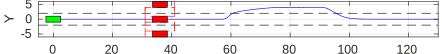
\includegraphics[width=1\columnwidth]{./figure/three_obstacles_no_overtaking/braking_0.pdf}
	\end{minipage}
	\begin{minipage}[t]{\columnwidth}
		\includegraphics[width=1\columnwidth]{./figure/three_obstacles_no_overtaking/braking_1.pdf}
	\end{minipage}
	\begin{minipage}[t]{\columnwidth}
		\includegraphics[width=1\columnwidth]{./figure/three_obstacles_no_overtaking/braking_2.pdf}
	\end{minipage}
%	\begin{minipage}[t]{\columnwidth}
%		\includegraphics[width=1\columnwidth]{./figure/three_obstacles_no_overtaking/braking_3.pdf}
%	\end{minipage}
	\begin{minipage}[t]{\columnwidth}
		\includegraphics[width=1\columnwidth]{./figure/three_obstacles_no_overtaking/braking_4.pdf}
	\end{minipage}
%	\begin{minipage}[t]{\columnwidth}
%		\includegraphics[width=1\columnwidth]{./figure/three_obstacles_no_overtaking/braking_5.pdf}
%	\end{minipage}
	\begin{minipage}[t]{\columnwidth}
		\includegraphics[width=1\columnwidth]{./figure/three_obstacles_no_overtaking/braking_6.pdf}
	\end{minipage}	
	\vspace{-23pt}
	\caption{Simulation of braking and overtaking obstacles.}
	\label{fig:braking}
\end{figure}
%\vspace{-12pt}
%
\subsubsection{Vehicle Braking and Obstacles Overtaking}
Finally we have improved the code related to the mixed Input/Output constraints so that in the case there are 3 obstacles that block the road and drive at a lower speed than the ATLASCAR2, the velocity of the vehicle decreases in order to prevent the collision. Figure \ref{fig:braking} depicts a simulation in which there are 3 obstacles at the same $x$-coordinate. Two obstacles have a constant speed of \SI{8}{m/s} while the one on the left lane of \SI{15}{m/s}.

At the beginning, the vehicle detects all the other cars on the road. In the first part of the simulation, the ATLASCAR2 brakes because there is not enough space for overtaking the cars as shown in Fig. \ref{fig:velocity_braking}. A collision would happen if the vehicle continues to follow the initially planned path with the reference velocity. It is possible to notice that the speed decreases because the applied throttle is negative, so a consistent deceleration is set after $\approx\SI{1.5}{s}$ as depicted in Fig. \ref{fig:throttle_braking}. After a few seconds the fastest obstacle moves and makes available the left lane. Dramatic changes of steering angle in early stage are observed in Fig. \ref{fig:delta_braking} and consequently also on the heading angle in Fig. \ref{fig:theta_braking}. Then, the ATLASCAR2 returns to the reference velocity during the overtaking of the two obstacles. It is seen that the ATLASCAR2 avoids the obstacles and returns to the road center line with a low overshoot.
\begin{figure*}[!t] %vs changes to t instead of b
	\vspace{-1.7em}
	\begin{minipage}[t]{\columnwidth}
		\includegraphics[width=\columnwidth,height=0.5\columnwidth]{./figure/three_obstacles_no_overtaking/VelocityVsTime.pdf}
		\vspace{-17pt}
		\subcaption{}\label{fig:velocity_braking}
	\end{minipage}
	\hfill
	\begin{minipage}[t]{\columnwidth}
		\includegraphics[width=\columnwidth,height=0.5\columnwidth]{./figure/three_obstacles_no_overtaking/ThrottleVsTime.pdf}
		\vspace{-17pt}
		\subcaption{}\label{fig:throttle_braking}
	\end{minipage}
		\vspace{-0.5em}
	\begin{minipage}[t]{\columnwidth}
	    \includegraphics[width=\columnwidth,height=0.5\columnwidth]{./figure/three_obstacles_no_overtaking/SteeringAngleVsTime.pdf}
	    \vspace{-17pt}
	    \subcaption{}\label{fig:delta_braking}
	\end{minipage}
	\hfill
	\begin{minipage}[t]{\columnwidth}
	    \includegraphics[width=\columnwidth,height=0.5\columnwidth]{./figure/three_obstacles_no_overtaking/HeadingAngleVsTime.pdf}
	    \vspace{-17pt}
	    \subcaption{}\label{fig:theta_braking}
	\end{minipage}
	\caption{Time signals of the ATLASCAR2 in the simulation of braking and overtaking in the situation illustrated in Fig. \ref{fig:braking}.}
	\label{fig:components}
\end{figure*}

\section{Conclusions and Future Work}
This paper proposes an advanced method for short term motion planning of an autonomous car based on adaptive Model Predictive Control. The central component is an obstacle avoidance system that moves the vehicle around different moving obstacles in the lane using throttle and steering angle. This system updates both the predictive model and the mixed input/output constraints at each control interval. The vehicle is also able to brake in order to prevent collisions against closest obstacles.
The flexibility of the concepts used in the algorithm allows a multitude of refinements and extensions to this work. We can add to this algorithm a lane following system that keeps the ATLASCAR2 traveling along the center line of the lanes on the road by adjusting the front steering angle of the car. The future work includes the combination of these two control strategies in a way that they can operate simultaneously. Next expected steps include the migration to ROS-Gazebo simulation environment and, later on, the usage of real data collected on board the ATLASCAR2 and, ultimately, test it in a real autonomous driving scenario.

\balance

\begin{thebibliography}{00}
	
	\bibitem{RRT}Kuwata, Y., Fiore, G. A., Teo, J., Frazzoli, E., and How, J. P., “Motion Planning for Urban Driving using RRT,” Proceedings of the IEEE International Conference on Intelligent Robots and Systems, Nice, France: 2008, pp. 1681–1686.
	
	\bibitem{potential}Lei Tang, Songyi Dian, Gangxu Gu, Kunli Zhou, Suihe Wang and Xinghuan Feng, "A novel potential field method for obstacle avoidance and path planning of mobile robot," 2010 3rd International Conference on Computer Science and Information Technology, Chengdu, 2010, pp. 633-637.
	
	\bibitem{meta-heuristic}Hussein, H. Mostafa, M. Badrel-Din, O. Sultan, and A. Khamis, "Metaheuristic optimization approach to mobile robot path planning," in 1st International Conference on Engineering and Technology (ICET), New Cairo, Egypt, 2012.
	
	\bibitem{borelli2}Y. Gao, T. Lin, F. Borrelli, E. Tseng, and D. Hrovat, "Predictive control of autonomous ground vehicles with obstacle avoidance on slippery roads," in Proceedings of Dynamic Systems and Control Conference (DSCC), 2010.
	
	\bibitem{nonlinearmpc}L. Grune and J. Pannek, in Nonlinear Model Predictive Control: Theory and Algorithms. Springer London, 2011, pp. 43-66
	
	\bibitem{skoda}J. Škoda, ‘3D Navigation for Mobile Robots’, Dissertation, 2017.
	
	\bibitem{fuzzyMPC}Y. Nishio, K. Nonaka and K. Sekiguchi, "Moving obstacle avoidance control by fuzzy potential method and model predictive control," 2017 11th Asian Control Conference (ASCC), Gold Coast, QLD, 2017, pp. 1298-1303.
	
	\bibitem{NONMPC}Yu, S., Li, X., Chen, H. and Allgöwer, F. (2015), "Nonlinear model predictive control for path following problems". Int. J. Robust Nonlinear Control, 25: 1168–1182. 
	
	\bibitem{safety}T. Xu and H. Yuan, "Autonomous vehicle active safety system based on path planning and predictive control," 2016 35th Chinese Control Conference (CCC), Chengdu, 2016, pp. 8889-8895.
	
	\bibitem{archi}M. Nolte, M. Rose, T. Stolte and M. Maurer, "Model predictive control based trajectory generation for autonomous vehicles — An architectural approach," 2017 IEEE Intelligent Vehicles Symposium (IV), Los Angeles, CA, 2017, pp. 798-805.
	
	\bibitem{MMPC}J. Ji, A. Khajepour, W. W. Melek and Y. Huang, "Path Planning and Tracking for Vehicle Collision Avoidance Based on Model Predictive Control With Multiconstraints," in IEEE Transactions on Vehicular Technology, vol. 66, no. 2, pp. 952-964, Feb. 2017.
	
	\bibitem{autoMPC}J. V. Frasch et al., "An auto-generated nonlinear MPC algorithm for real-time obstacle avoidance of ground vehicles," 2013 European Control Conference (ECC), Zurich, 2013, pp. 4136-4141.
	
	\bibitem{borelli}V. Turri, A. Carvalho, H. E. Tseng, K. H. Johansson and F. Borrelli, "Linear model predictive control for lane keeping and obstacle avoidance on low curvature roads," 16th International IEEE Conference on Intelligent Transportation Systems (ITSC 2013), The Hague, 2013, pp. 378-383.	
	
%	\bibitem{atlas}ATLAS  Project,  Aveiro  University, Portugal, \url{http://atlas.web.ua.pt/}, last visited July 2010.
		

	\bibitem{atlascar1}V. Santos et al., "ATLASCAR - technologies for a computer assisted driving system on board a common automobile", 13th International IEEE Conference on Intelligent Transportation Systems, Funchal, 2010, pp. 1421-1427.
		
	\bibitem{atlascar2}V. Santos, "ATLASCAR: A Sample of the Quests and Concerns for Autonomous Cars", Informatics in Control, Automation and Robotics: 14th International Conference, ICINCO 2017 Madrid, Spain, Revised Selected Papers (in press March 2019).
		
    \bibitem{ricardo}R. Silva, "Navegação Local do ATLASCAR2 para Condução Autónoma e Assistência ao Condutor", Dissertação de mestrado. Departamento de Engenharia Mecanica, Universidade de Aveiro, 2018.
    
	\bibitem{siciliano}B. Siciliano, L. Sciavicco, L. Villani, and G. Oriolo. "Robotics: Modelling, Planning and Control", Springer Publishing Company, Incorporated, 2008. 
%	\bibitem{onlineMPC}M. Werling and D. Liccardo, "Automatic collision avoidance using model-predictive online optimization," 2012 IEEE 51st IEEE Conference on Decision and Control (CDC), Maui, HI, 2012, pp. 6309-6314.
	
	\bibitem{swarms}Wei Xi and J. S. Baras, "MPC based motion control of car-like vehicle swarms," 2007 Mediterranean Conference on Control \& Automation, Athens, 2007, pp. 1-6.
	
	
	\bibitem{long_tf}Y. Wang, Y. Bin and K. Li, "Longitudinal acceleration tracking control of low speed heavy-duty vehicles," in Tsinghua Science and Technology, vol. 13, no. 5, pp. 636-643, Oct. 2008.
	
	\bibitem{mpctoolbox}A. Bemporad, M. Morafi, and N. Ricker, Model Predictive Control Toolbox User’s Guide, The MathWorks, Inc.,
	
		\url{https://www.mathworks.com/help/pdf_doc/mpc/mpc_ug.pdf}
		
%	\bibitem{theory}J. Rawlings, D. Mayne (2010), "Model Predictive Control: Theory and Design", Nob Hill Publishing.	
	
%	\bibitem{backward}C. Son and C. Ahn, "Vehicle backward driving control with obstacle avoidance," 2015 15th International Conference on Control, Automation and Systems (ICCAS), Busan, 2015, pp. 1771-1774.
	
	
%	\bibitem{zhou}H. Zhou, L. Güvenç and Z. Liu, "Design and evaluation of path following controller based on MPC for autonomous vehicle," 2017 36th Chinese Control Conference (CCC), Dalian, 2017, pp. 9934-9939.
	
%	\bibitem{yu} Z. T. Yu, Obstacle Avoidance for Autonomous Vehicle Driving on Highways Based on MPC, JinLin University, 2012.
	
%	\bibitem{berger}Berger, Niels. (2018). Lane Change Path Planning With state-dependent safety constraints using Nonlinear Model Predictive Control.
	
%	\bibitem{kth_thilen}E. Thilén, ‘Robust Model Predictive Control for Autonomous Driving’, Dissertation, 2017.
	
%	\bibitem{rathai}Murali Madhavan Rathai, Karthik \& Amirthalingam, Jegan \& Jayaraman, Balaji. (2017). Robust tube-MPC based lane keeping system for autonomous driving vehicles. 1-6.
	
	
%	\bibitem{kth_nordell}B. Nordell, ‘Trajectory Planning for Autonomous Vehicles and Cooperative Driving’, Dissertation, 2016.
	
%	\bibitem{shen}C. Shen, H. Guo, F. Liu and H. Chen, "MPC-based path tracking controller design for autonomous ground vehicles," 2017 36th Chinese Control Conference (CCC), Dalian, 2017, pp. 9584-9589.
	
%	\bibitem{matsumoto}N. Wada and T. Matsumoto, "Driver assistance for collision avoidance by constrained MPC," 2017 56th Annual Conference of the Society of Instrument and Control Engineers of Japan (SICE), Kanazawa, 2017, pp. 90-93.
		
\end{thebibliography}


\end{document}